\chapter{Literature}
\label{background}

\section{Programming Assessment}
In {\it Automated Evaluation of Programming Assignments}\cite{automate_evaluation}, Kaushal and Singh describe various measures used as part of an automated marking system: regularity, integrity, efficiency and accuracy. 
\paragraph*{Regularity} The time at which a submission is made with respect to the deadline for that submission
\paragraph*{Integrity} The originality of the document determined through a plagiarism detector
\paragraph*{Efficiency} A qualitative measure of the time taken and memory used by a student's programs
\paragraph*{Accuracy} The percentage of test cases for each program that the student's submission passes

The experimenters track the change in these measures as students use the system and find that there is a general improvement on all categories when feedback is based on these measurements. This shows that accuracy is not the only measurement that should be used to provide feedback and these are possibilities to be considered for Infandango. Currently the only feedback Infandango provides is based on accuracy, so creating a form of feedback capable of considering these other areas could be worthwhile.

\section{Visualisation}
In his book {\it Visual Display of Quantitative Information}\cite{visual_explanations}, Edward Tufte discusses methods of efficiently and effectively displaying information. In chapter 4 Data-Ink and Graphical Redesign, Tufte introduces the idea of Data-Ink: The amount of "ink" which is actually used to represent the data you are interested in. In Tufte's words:

\begin{quote}Data-ink is the non-erasable core of a graphic, the non-redundant ink arranged in reponse to the variation in the numbers represented.
\end{quote}
Data-ink is desirable, unavoidable information so Tufte says designers should strive towards a high data-ink ratio, removing as much non-information ink as possible to avoid overwhelming the data. Tufte then continues by giving examples where redundant information is desirable. One of these examples uses a graphic from Linus Pauling's General Chemistry (San Francisco, 1947) p64. Figure \ref{fig:tuftegraphs} shows how, based on the low data-ink ratio principle, he removes the grid marks and part of the frame which leaves little else but the data itself.

\begin{figure}[h!]
\centering
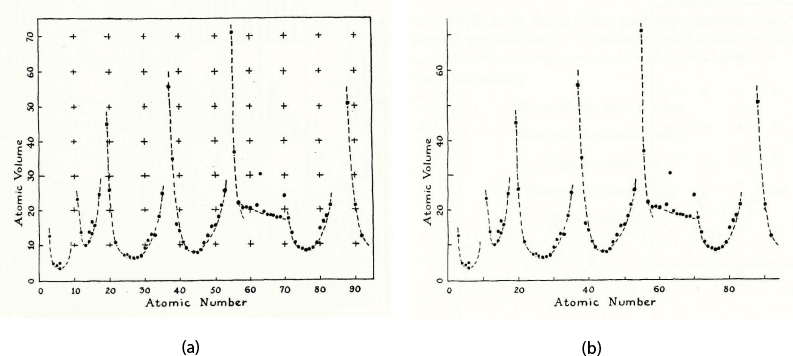
\includegraphics[width=0.8\textwidth]{images/tuftegraphs.png}
\caption{(a) shows the original graph and (b) shows how Tufte recommends changing the graph to remove redundant information}
\label{fig:tuftegraphs}
\end{figure}


Tufte concludes the chapter with 5 maxims summarising this principle.

\begin{verse}
	Above all else show the data.
	Maximize the data-ink ratio.
	Erase non-data-ink.
	Erase redundant data-ink.
	Revise and edit.
\end{verse}

There are principles which Infandango currently adheres to quite well. For example, the score which is provided for each question is displayed as a percentage on a block of colour which depends on the score. At first the block of colour may seem redundant since it is a feature related directly to the score so it doesn't seem to add much information. However, the score alone would not tell the user if that score is "good" or "bad", that is a judgement the user would have to make for themselves. Providing this information as a colour is a simple, intuitive way of telling the use whether their performance on an exercise is acceptable or not.

\section{Cognitive Modelling}
The cognitive modelling of students can provide access to important information for automatic tutoring systems. A cognitive model is a computer model of the cognitive processes of a student, which allows insight into how the student might approach the problem, or how difficult the problem might be for the student. Building this model manually requires a lot of human effort\cite{simstudent_better} and so automating this process is desirable.

SimStudent is a machine learning agent designed to build cognitive models automatically via machine learning. The machine learning method used for parts of SimStudent is a First Order Inductive Learner, which is given some some observations and background knowledge from which it draws hypotheses. Using algebra as an example, SimStudent will be given some basic operators as background knowledge (add, subtract etc) and will then be given an algebraic problem to solve. It will then suggest the next step to the student who may reject or accept the suggestion, thus providing negative or positive feedback to SimStudent to modify its production rules.

As long as the students perform consistently, SimStudent can model the performance of the students with an accuracy of 83\%\cite{simstudent}. Being able to model and predict a student's performance can allow the tutoring system to target feedback at the areas which it knows the student might struggle with, thus catching problems before they occur and understanding why certain mistakes happen.

\section{Machine Learning and Feedback for an Online Marking System}
Khan Academy\cite{khan_site} is a website which provides users with online education material:
\begin{quote}
Our online materials cover subjects ranging from math and finance to history and art.  With thousands of bite-sized videos, step-by-step problems and instant data\cite{ka_faq}
\end{quote}

\begin{figure}[h!]
\centering
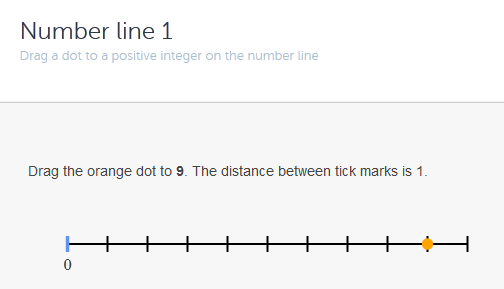
\includegraphics[width=0.8\textwidth]{images/kascreenshot.png}
\caption{A screenshot of the online Khan Academy system, showing a simple exercise where the user must choose the correct position on a number line.}
\label{fig:kascreenshot}
\end{figure}

A blog post\cite{khan_blog} written by David Hu about Khan Academy explains how they went about changing their feedback system. Khan Academy gives users certain kinds of exercises, for example choosing the approriate position on a number scale (see Figure \ref{fig:kascreenshot}. It can then generate endless variations of this problem for the user to continue attempting until they are deemed proficient. Proficiency is the phrase used by Khan Academy which the user is good enough at the exercise that they should move on. The original Khan Academy system required the user to get 10 consecutive exercises of a certain type correct before they are qualified as proficient for that type of exercise. 

The main problem with this system is that a user could get 9 consecutive exercises correct and then make a mistake on the final exercise. Before the user could move on they would have to get 10 more consecutive exercises correct. Hu decided it would be better if the system took into account how the user had performed previously. 

In an attempt to improve this system Hu proposed using a logistic regression model to calculate the probability that a user passes the next exercise successfully, with a threshold of 94\% representing the new proficiency level. Over a 6 day period 10\% of users tested the new method. Users of the new system earned 20.8\% more proficiences, attempted 15.7\% more exercises and required 26\% less exercises per proficiency. Hu summarises by saying the boost seems to come from allowing users to move on from exercises which they are already proficient at, without requiring them to complete their streak.

Although the current Infandango system does not require perfection like Khan Academy did, it is possible that users are more reluctant to move on from exercises before they achieve 100\%, since in a task such as programming, where the tests are strict and objective, it is very possible and common to get 100\%. Encouraging the user to move on when they do not yet have 100\% could provide increase in the performance of the students.


\section{Conclusion}
The literature provides a strong case for applying machine learning to the problem of improving automated feedback. Infandango currently lacks feedback which uses information from multiple exercises, and doing so may allow more detailed and targeted feedback. While cognitive modelling is effective, it is more suited to rule based learning, where logic can be applied to the knowledge in order to learn hypotheses. The Khan Academy approach is more applicable to Infandango as it only needs to know the mark for an exercise, not the rules which a student applies in order to solve the exercise.
